\chapter{DESAIN DAN IMPLEMENTASI}
\label{chap:design-and-implementation}

% Ubah bagian-bagian berikut dengan isi dari desain dan implementasi

Bab ini menjelaskan desain dan implementasi dari sistem yang telah dibuat.
Seperti yang terlihat pada Gambar \ref{fig:block-diagram}, terdapat 2 diagram blok utama. Di bagian kiri adalah diagram blok untuk mode \textit{RECORD} dan diagram blok kanan adalah untuk mode \textit{PLAY}.
Pada mode \textit{RECORD}, dimulai dengan citra manusia yang menjadi input ke estimasi pose untuk mendapatkan \textit{keypoint} manusia.
Setelah itu, melakukan konversi sudut antara 2 \textit{keypoint} menjadi nilai servo sehingga dapat menggerakkan servo-servo robot untuk menirukan gerakan manusia serta menyimpannya untuk mode \textit{PLAY}.
Di sisi lain, input pada mode \textit{PLAY} terdiri dari 2 yaitu citra manusia dan citra robot \textit{humanoid}.
Kemudian, dilakukan estimasi pose untuk kedua citra tersebut. Sebelum melakukan normalisasi \textit{keypoint}, dilakukan pemilihan 6 \textit{keypoint} manusia berdasarkan \textit{keypoint} robot \textit{humanoid}.
Terakhir, membandingkan \textit{keypoint} tersebut serta mendapatkan hasilnya.
\begin{figure}[ht]
  \centering
  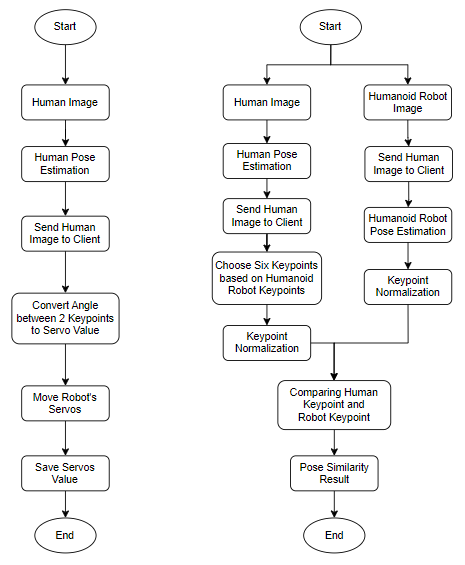
\includegraphics[scale=1.2]{gambar/diagram-block-revisi.png}
  \caption{Blok Diagram dari Alur Pengerjaan.}
  \label{fig:block-diagram}
\end{figure}
Pada bagian berikutnya, setiap blok akan dijelaskan secara lebih rinci. Perlu diperhatikan bahwa mungkin ada penjelasan yang digabung jika kita menggunakan teknik yang sama untuk blok yang berbeda.
Misalnya, blok yang mengirimkan citra manusia ke klien dan blok yang mengirimkan citra robot ke klien akan digabung menjadi hanya mengirimkan citra ke klien.


\section{Citra Input}
\label{sec:input-image}

Citra input yang dimasukkan ke dalam dua model (manusia dan robot \textit{humanoid}) memiliki ukuran 640x480 piksel dengan saluran RGB.
Perangkat yang digunakan untuk mendapatkan citra adalah Logitech C920 Webcam. Kami menggunakan \textit{library} OpenCV untuk membuka kamera dan mengambil citra.


\section{Estimasi Pose Manusia}
\label{sec:estimasi-pose-manusia}

Dikarena sudah banyaknya model estimasi pose untuk manusia yang tersedia, kami tidak perlu melakukan pelatihan ulang dan hanya membandingkannya untuk mencari model terbaik melalui referensi dari beberapa makalah.
Metrik evaluasi berdasarkan paper dan hasil deteksi setiap model akan ditunjukkan pada Bab \ref{chap:resultsandiscussion}, namun untuk waktu inferensi akan dicoba pada NUC i5.
Model-model yang dibandingkan adalah OpenPose, MediaPipe Pose, dan YOLO-pose. Input untuk model-model ini adalah citra RGB lalu outputnya adalah lokasi \textit{keypoint} manusia.

\section{Mengirim Citra ke Klien}
\label{sec:send-image-to-client}

Program utama kami menggunakan website untuk berinteraksi dengan pengguna karena fleksibilitasnya pada berbagai \textit{platform}, tampilan website dapat dilihat pada Gambar \ref{fig:websiteview}. 
Akan ada klien Javascript dan Server Python yang berkomunikasi melalui \emph{socketio}.
Server akan mengirimkan citra manusia ke klien sehingga kita dapat menyesuaikan posisi kita di depan kamera. Hal ini dilakukan agar robot dapat mengambil seluruh pose manusia.
\begin{figure}[ht]
  \centering
  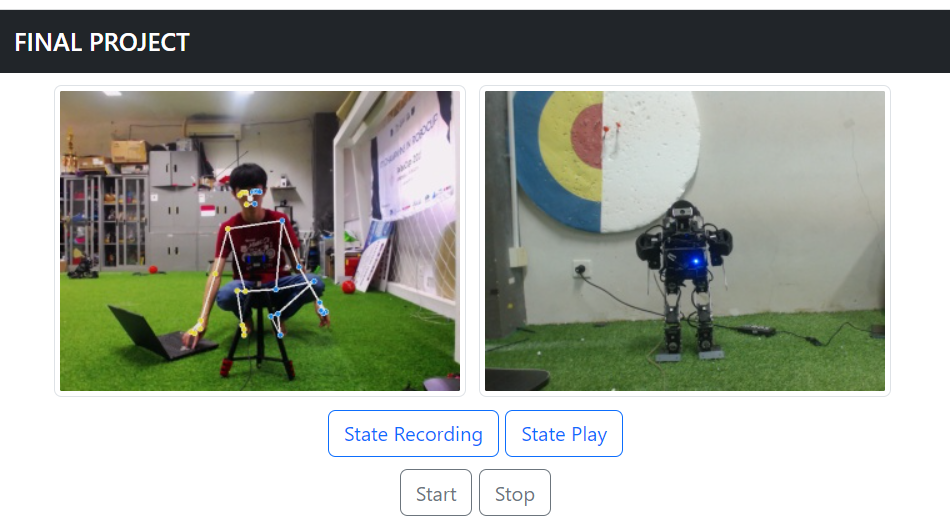
\includegraphics[scale=0.7]{gambar/web.png}
  \caption{Tampilan Website.}
  \label{fig:websiteview}
\end{figure}
Program utama ini terbagi menjadi dua mode, yaitu mode \textit{RECORD} dan mode \textit{PLAY}. Pada mode \textit{RECORD}, manusia berperan sebagai pelatih dan memberikan serangkaian gerakan yang akan ditiru oleh robot \textit{humanoid} serta gerakan tersebut akan disimpan oleh robot untuk digunakan di mode \textit{PLAY} nantinya.
Sementara itu, pada mode \textit{PLAY}, robot bertindak sebagai pelatih dan memperagakan serangkaian gerakan sesuai yang disimpan pada mode \textit{RECORD}. Manusia akan meniru gerakan robot selagi robot juga menyimpan citra manusia dan citra robot lalu membandingkannya nanti.

Setelah mendapatkan \textit{keypoint} manusia, server akan memvisualisasikan hasil deteksinya dan mengirimkan sebagai buffer ke klien.
Di sisi klien, kami menggunakan \textit{library ReactJS}. Terdapat empat tombol: tombol \textit{RECORD}, \textit{PLAY}, \textit{START}, dan \textit{STOP}. Tombol \textit{RECORD} dan \textit{PLAY} mengindikasikan mode dalam program utama, sementara tombol \textit{START} dan \textit{STOP} memberitahu kapan mode dimulai atau dihentikan.
Setelah mengklik tombol, tombol tersebut akan berubah warna untuk menunjukkan bahwa tombol tersebut sudah ditekan.
Selain itu, terdapat dua citra yang menampilkan citra manusia dan robot. Sebenarnya, pada mode \textit{RECORD} hanya ada satu citra (citra manusia), sedangkan pada mode \textit{PLAY} terdapat 2 citra (citra manusia dan citra robot).
Klien dan server berkomunikasi melalui port 5555, di mana server dapat mengirim citra ke klien dan klien dapat mengirim beberapa data kembali ke server seperti mode saat ini dan waktu untuk memulai atau menghentikan mode.
Kami menggunakan fungsi \emph{useEffect} untuk mengindikasi jika terdapat perubahan pada variabel tertentu dan melakukan sesuatu seperti mengonversi citra dari buffer menjadi \textit{string} untuk ditampilkan pada tag HTML.


\section{Konversi Sudut ke Nilai Servo}
\label{sec:convert-angle-to-servo-value}

Bagian ini dan Bagian \ref{sec:move-robot-servo} dijalankan ketika tombol \textit{RECORD} dan \textit{START} ditekan pada website, sehingga klien mengirimkan informasi ini ke server dan server melakukan perhitungan.
Untuk dapat menggerakkan tubuh bagian atas robot sesuai dengan gerakan manusia, kita perlu mendapatkan sudut antara 2 \textit{keypoint} menggunakan fungsi \emph{arc tangent} dengan input koordinat \textit{keypoint} \emph{{x, y}}
DiKarenakan kami menggunakan MediaPipe Pose untuk mendeteksi \textit{keypoint} manusia berdasarkan hasil dan pembahasan di Bagian \ref{sec:humanmodelcomparison}, outputnya adalah titik yang ternormalisasi, jadi harus dilakukan pengkalian koordinat x dan y dengan lebar dan tinggi gambar masing-masing untuk mendapatkan nilai piksel yang sebenarnya.
Selanjutnya, kita membagi nilai \textit{keypoint} y dengan nilai \textit{keypoint} x serta menginputkan hasilnya ke fungsi \emph{arc tangent}, seperti yang ditunjukkan dalam Persamaan \ref{eq:arctan}.
\begin{equation}
  \label{eq:arctan}
  angle = \arctan \left(\frac{Y_2 - Y_1}{X_2 - X_1}\right)
\end{equation}

Ada empat sudut yang ingin diperoleh, yaitu sudut dari bahu ke siku (kanan dan kiri) dan juga siku ke pergelangan tangan (kanan dan kiri) agar robot dapat meniru gerakan bagian atas tubuh manusia.
Jika kita melihat MediaPipe Pose Landmark pada Gambar \ref{fig:mediapipe-landmark}, 6 \textit{keypoint} yang menjadi perhatian adalah 11, 12 untuk bahu, 13, 14 untuk siku, 15, dan 16 untuk pergelangan tangan.
Kita mendapatkan nilai sudut bahu kanan dengan memasukkan landmark 14 sebagai argumen kedua dan landmark 12 sebagai argumen pertama dari fungsi \emph{arc tangent}. Hal yang sama juga berlaku untuk mendapatkan nilai sudut bahu kiri dengan memasukkan landmark 13 dan 11 secara berurutan.
Hal ini sedikit berbeda untuk mendapatkan sudut siku karena kita ingin sudutnya relatif terhadap sudut bahu dengan mengurangi sudutnya dari sudut bahu.
Kami juga memberlakukan batasan untuk setiap sudut untuk menjaga keamanan servo dan menghindari benturan dengan tubuh robot atau servo lainnya seperti yang terlihat pada Tabel \ref{tb:robot-servos}.
\begin{longtable}{ccc}
  \caption{Limitasi Servo Robot.}
  \label{tb:robot-servos}\\
  \hline
  \rowcolor[HTML]{C0C0C0}
  \textbf{Joint Angle} & \textbf{Motion} & \textbf{Range (deg)} \\
  \hline
  LShoulderRoll       & Left shoulder joint right and left    & -110 to 30  \\
  RShoulderRoll       & Right shoulder joint right and left   & -30 to 110 \\
  \rowcolor[HTML]{C0C0C0}
  \textbf{Joint Angle} & \textbf{Motion} & \textbf{Range (deg)} \\
  \hline
  LElbowPitch           & Left Elbow joint front and back       & -120 to 10  \\
  RElbowPitch           & Left Elbow joint front and back       & -10 to 120  \\
  \hline
\end{longtable}


\section{Menggerakkan Servo-servo Robot}
\label{sec:move-robot-servo}

Program untuk menggerakkan servo robot berada di tempat yang sama dengan program untuk \textit{server}. Program utama kami menggunakan ROS2 dengan bahasa Python. Untuk dapat menjalankan program \textit{server} dan program ROS2 secara bersamaan, kami membutuhkan \textit{thread} terpisah sehingga program \textit{server} tidak menghalangi ROS2.
Dalam \textit{framework} ROS2, setiap \textit{package} memiliki fungsionalitasnya masing-masing. Pada kesempatan ini, kami membagi tugas untuk menggerakkan servo robot menjadi 2 \textit{package}. Yang pertama bernama \emph{motion matching} di mana program server dan konversi sudut menjadi nilai servo terjadi, yang satunya lagi adalah \emph{tachimawari}, sebuah \textit{package} yang menyediakan \textit{management library} sendi DYNAMIXEL untuk proyek ROS 2.
Nama paket ini berasal dari kata bahasa Jepang yang berarti \textit{motion}. Setiap \textit{package} memiliki sebuah \textit{node} dengan nama \textit{package} itu sendiri seperti yang terlihat pada Gambar \ref{fig:relation-node-record-mode}.
Hubungan antar node ini dapat dilihat melalui grafik rqt atau \textit{ROS2 client interfaces}, tetapi kami memilih grafik rqt karena lebih visual.
\begin{figure}[ht]
  \centering
  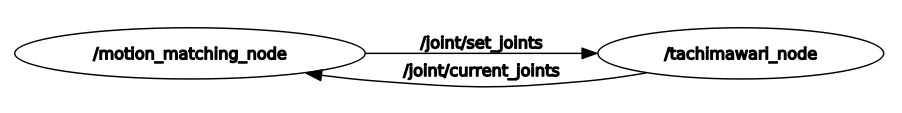
\includegraphics[scale=0.62]{gambar/rqt_without_akushon.png}
  \caption{Hubungan Antar \textit{Node} pada mode \textit{RECORD}.}
  \label{fig:relation-node-record-mode}
\end{figure}

Setiap \textit{node} berkomunikasi satu sama lain melalui topik. Terdapat 2 topik dalam mode \textit{RECORD}, yaitu \verb|joint/set_joints| dan \verb|joint/current_joints|.
Setelah mendapatkan sudut servo yang diinginkan dari bagian sebelumnya, kita hanya perlu mem-\textit{publish} ke \emph{tachimawari node} dan \textit{node} tersebut akan menggerakkan servonya. Di dalam \emph{motion matching node}, terdapat sebuah \emph{publisher} yang mem-\textit{publish} sudut servo ke topik \verb|joint/set_joints| setelah proses deteksi dan
perhitungan selesai dilakukan, serta terdapat \emph{subscriber} pada \emph{tachimawari node} yang mendengarkan pada topik yang sama untuk mengumpulkan data yang di-\textit{publish} oleh \emph{publisher}. Topik \verb|joint/set_joints| menggunakan antarmuka seperti yang terlihat pada potongan kode \ref{lst:set-joint-msg}, di mana terdapat variabel \verb|control_type| dengan tipe data \textit{integer} dan sebuah array dengan tipe \textit{Joint}, setiap \textit{Joint} terdiri dari \textit{id} dan \textit{position} seperti pada potongan kode \ref{lst:joint-msg}.
\begin{lstlisting}[
  language={},
  caption={\textit{Joint msg}.},
  label={lst:joint-msg}
]
uint8 id
float32 position
\end{lstlisting}

\begin{lstlisting}[
  language={},
  caption={\textit{SetJoints msg}.},
  label={lst:set-joint-msg}
]
int8 control_type 4
Joint[] joints
\end{lstlisting}

Di dalam \verb|tachimawari_node| terdapat \verb|joint_node| yang mempublikasikan nilai sendi saat ini setiap 8ms (akan digunakan pada bagian berikutnya) dan memiliki \emph{subscriber} yang mendengarkan sendi yang ingin kita gerakkan.
Untuk dapat menggerakkan servonya ke nilai yang diinginkan, kita harus mengaktifkan \emph{torque} dari semua servo terlebih dahulu. Kemudian kita membuat sebuah perintah dalam bentuk \textit{array} yang berisi \textit{id} servo dan nilai yang diinginkan atau nilai target kita (16 \textit{byte}) yang dibagi menjadi 2 * 8 \textit{byte}.
Sebagai contoh, nilai target kita adalah 512 (dalam bentuk biner sama dengan \verb|00000010 00000000|), pesan yang kita kirim adalah 2 (\verb|00000010|) dan 0 (\verb|00000000|). Hal ini dapat kita peroleh dengan melakukan operasi \textit{bitwise AND} dan \textit{bitwise right shif}t. Operasi \textit{bitwise AND} dilakukan antara nilai target dan \verb|0xFF|, yang direpresentasikan sebagai (\verb|00000000 11111111|) dalam bentuk biner.
Karena \verb|0xFF| memiliki 0 \textit{bit} di \textit{byte} yang lebih tinggi dan 1 \textit{bit} di \textit{byte} yang lebih rendah, hasil dari operasi tersebut adalah \textit{byte} yang lebih rendah dari nilai target. Di sisi lain, operator \textit{bitwise right shift} digunakan untuk menggeser \textit{bit-bit} servo target 8 posisi ke kanan. Menggeser \textit{bit} ke kanan sejauh 8 posisi secara efektif menghilangkan \textit{byte} yang lebih rendah, sehingga hanya \textit{byte} yang lebih tinggi yang tersisa dalam hasilnya.
Hal ini juga berlaku ketika kita menerima nilai posisi servo saat ini, servo juga mengirimkan data dalam bentuk dua \textit{byte} (\textit{byte} yang lebih rendah dan \textit{byte} yang lebih tinggi) dan kita perlu menggabungkan kedua \textit{byte} tersebut untuk merekonstruksi nilai 16-\textit{bit} yang mewakili posisi servo saat ini. Hal ini dapat dicapai dengan melakukan operasi \textit{left shift} pada \textit{byte} yang lebih tinggi.
Menggeser 8 \textit{bit} ke kiri secara efektif memindahkannya ke posisi \textit{byte} yang lebih tinggi. Setelah itu, operasi \textit{bitwise OR} menggabungkan \textit{byte} yang lebih tinggi yang telah digeser dengan \textit{byte} yang lebih rendah. Operasi ini menggabungkan kedua \textit{byte} tersebut untuk membentuk nilai 16-\textit{bit} yang mewakili posisi saat ini.


\section{Menyimpan Nilai Servo}
\label{sec:save-servo-value}

Pada bagian sebelumnya, kita telah membahas sedikit mengenai \emph{publisher} dalam \textit{package} \emph{tachimawari} yang mempublikasikan nilai setiap sendi saat ini dari robot melalui topik \verb|joint/current_joints|.
Terdapat juga \emph{subscriber} di dalam \verb|motion_matching| \textit{node} yang mengambil data tersebut, dan \textit{timer} ROS2 yang dijalankan setiap 0.5 detik untuk menyimpan \emph{current joints} saat ini dalam format JSON seperti pada potongan kode \ref{lst:json-save-joints}, sehingga robot dapat bergerak sesuai dengan gerakan yang diperagakan oleh manusia.
Format JSON yang disediakan mewakili objek data terstruktur yang menggambarkan tindakan atau urutan gerakan tertentu. Terdapat \textit{array} "\textit{poses}" yang berisi beberapa objek \textit{pose}, masing-masing mewakili konfigurasi \emph{joint} tertentu selama \textit{action} tersebut.
Setiap objek pose mencakup sub-objek "\textit{joints}", yang mencantumkan berbagai \emph{joint} dan nilai-nilai yang terkait. Misalnya, \verb|"left_ankle_pitch"| memiliki nilai 25, \verb|"left_ankle_roll"| diatur menjadi 0, dan seterusnya. Nilai-nilai ini mewakili posisi atau sudut dari \emph{joint} yang bersangkutan.
Setiap objek pose juga memiliki bagian "\textit{name}" untuk mengidentifikasi pose tersebut. Bagian "\textit{pause}" menentukan durasi jeda antara pose ini dan pose berikutnya, sedangkan "\textit{speed}" menunjukkan seberapa cepat pose ini akan dieksekusi.
Terakhir, bagian \verb|"start_delay"| menandakan jeda sebelum tindakan dimulai, dan bagian \verb|"stop_delay"| menandakan jeda setelah tindakan selesai sebelum robot berhenti. Secara keseluruhan, terdapat 20 servo pada robot, sehingga dalam file JSON yang sebenarnya, setiap sub-objek "\textit{joint}" memiliki 20 item dengan nama-nama \emph{joint} yang sesuai.
\begin{lstlisting}[
  language={},
  caption={Format JSON untuk Menyimpan Nilai Servo.},
  label={lst:json-save-joints}
]
{
  "poses": [
    {
      "joints": {
        "left_ankle_pitch": 25,
        "left_ankle_roll": 0,
      },
      "name": "pose name",
      "pause": 0,
      "speed": 0.003
    },
  ],
  "start_delay": 0,
  "stop_delay": 0
}
\end{lstlisting}


\section{Humanoid Robot Pose Estimation}
\label{sec:humanoid-robot-pose-estimation}

This explanation is intended for the right block diagram from Figure \ref{fig:block-diagram} or we can also say as the RECORD mode. The difference between the PLAY and RECORD modes lies in the number of cameras used.
So there will be two cameras, one camera to record human movement (located on the robot's head) and the other to record robot movement (located from the human side facing the robot), the distance between them approximately 1 - 1.5 meters, as shown in Figure \ref{fig:pose-comparison-side}.
In PLAY mode, the server side sends two images so that we can know and adjust the position of humans and robots in the camera. Due to the large network delay when sending two 320x240 pixel images, when the START button is pressed,
the server does not send the image to client again, the robot plays a series of moves stored in the previous JSON file by communicating via another ROS2 packages, while saving both images. After that, when the STOP button is pressed, the server starts to compare poses between them.
\begin{figure}[ht]
  \centering
  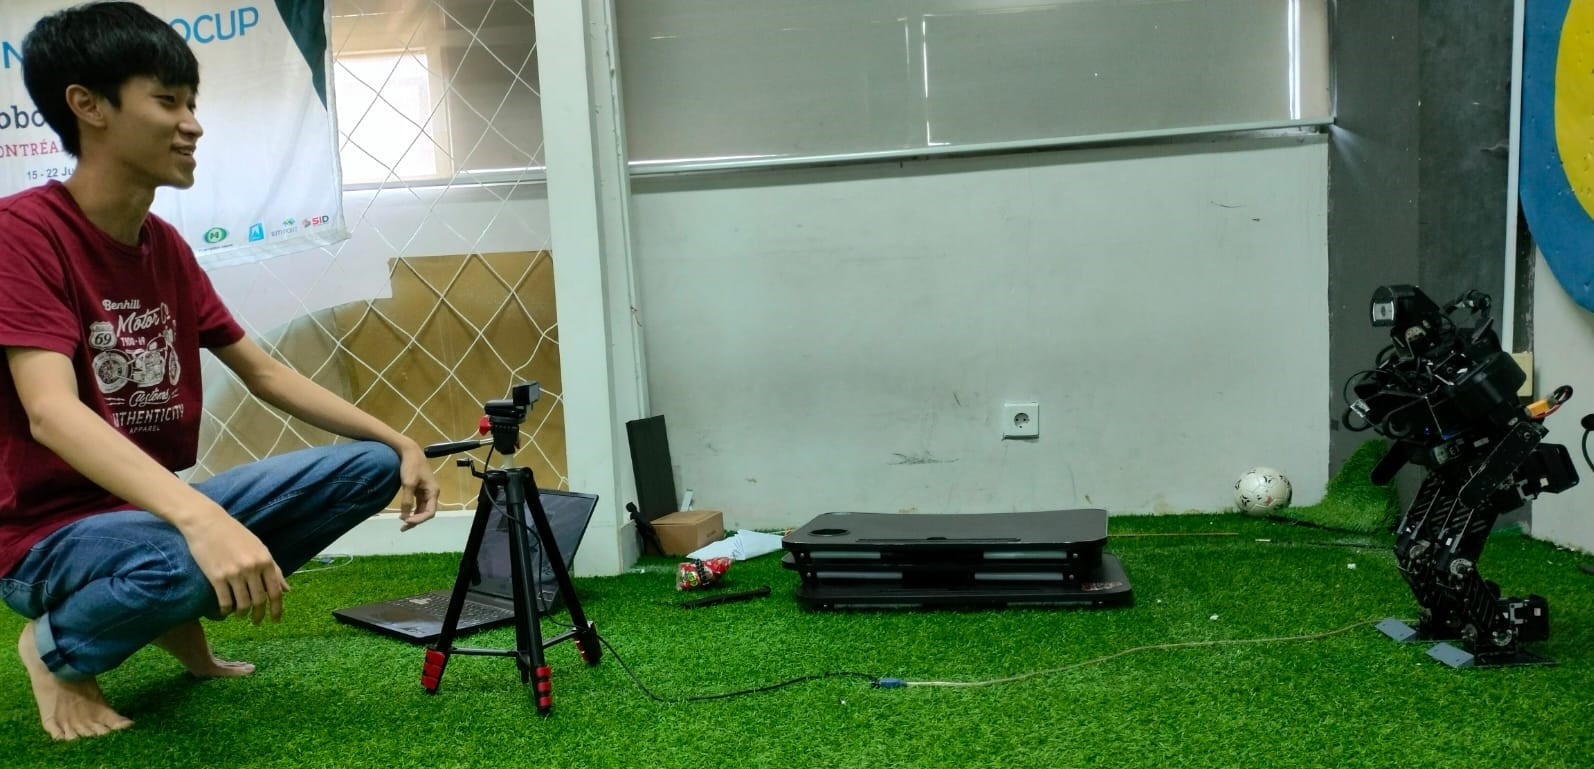
\includegraphics[scale=0.3]{gambar/pose-comparison.jpeg}
  \caption{Pose Comparison from Side.}
  \label{fig:pose-comparison-side}
\end{figure}

In order to move the servo robot according to the data stored in JSON, a package called \emph{akushon} is needed. \emph{Akushon} is a package related to motion robots. This package name comes from a Japanese word that means action.
Like Section \ref{sec:move-robot-servo}, every package has a node with the package's name and communicates with each other through a topic as shown in Figure \ref{fig:relation-node-play-mode}. There are 3 topics in PLAY mode: \verb|joint/set_joints|, \verb|joint/current_joints| that is used between \verb|akushon_node| and \verb|tachimawari_node| also \verb|motion_matching_node| and \verb|tachimawari_node|,
and \verb|action/run_action| that is used between \verb|akushon_node| and \verb|mo| \verb|tion_matching_node|.
The explanation about how to move the robot's servos and get the current value of servos through topic \verb|joint/set_joints| and \verb|joint/current_joints| is located in Section \ref{sec:move-robot-servo}.
Meanwhile, topic \verb|action/run_action| is used to send pose data in a JSON file from \emph{motion matching} to \emph{akushon} package. In \emph{akushon} package there is an interpolator that loops through every pose in the JSON file, get every value of the servo, and send it to \emph{tachimawari} package.
\begin{figure}[ht]
  \centering
  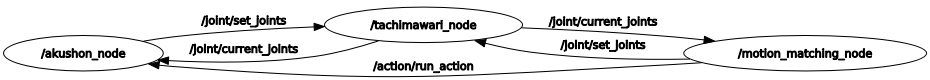
\includegraphics[scale=0.64]{gambar/rqt_akushon.png}
  \caption{Relationship Between Nodes in PLAY Mode.}
  \label{fig:relation-node-play-mode}
\end{figure}

This section immediately begins with the estimation pose for humanoid robot because the explanation regarding the previous block has been explained in the previous section.
Since there are not many pose estimation models for humanoid robots out there yet, we need to retrain them or use transfer learning from the model that supposes to estimate human pose.
Therefore, the following subsections will explain about the steps for training pose estimation on humanoid robot.

\subsection{Make New Dataset}
\label{subsec:make-new-dataset}

This new dataset is a merge of NimbRo's Humanoid Robot Pose dataset and Ichiro's dataset. NimbRo's dataset contains both single and multiple robots to
simulate RoboCup's real conditions. They also gathered from RoboCup Humanoid League YouTube videos, their own internal videos, and ROS bags. 
Overall, their dataset has over 1.5k images that come from 23 videos with around 2.3k robot instances. These images include teen and adult-sized robots and contain more than ten different robot types \parencite{amini2021}.
However, the robots in Ichiro's dataset are only kid-sized and come in single or maximum two-robot configurations. The images in our dataset come from videos that are taken in our lab. 
Then we split up those videos into multiple images and we pick not blurred videos.
Before merging, we need to fix NimbRo's dataset format first. This is because after we visualized some of their data, we found that the bounding boxes in \emph{annotations} part were misplaced (the width and height were swapped).
After we refine their dataset format and merge them with our dataset, the newly created dataset has approximately 2.1k images.
About 20 percent of the dataset was used for scoring and validating.

When it comes to annotation tools, there are a lot of choices out there including offline and online tools. We have tried some of them like Dataloop, V7labs, or Supervisely which is recommended by NimbRo.
However, when we tried to export the dataset into COCO format, it failed (e.g. can not import it or it can be imported but the JSON result in the annotation section is none). So, we decided to use a coco-annotator,
a web-based image annotation tool designed for versatility and efficiently labeling images to create training data. Regarding the number of keypoints in each robot, we followed NimbRo's dataset.
There are six keypoints including head, trunk, hands, and feet. We stick to that idea because we want to try the model's performance and inference time with fewer keypoints first and if we are confident enough, we will increase the number of keypoints later.

\subsection{Training Pose Estimation Model for Humanoid Robot}
\label{subsec:training-robot}

All of the training processes in this study were primarily conducted on a DGX-A100 server computer and written in the Python programing language. The specific configuration explains in Table \ref{tb:dgxa100}.
From this base specification, we are allocated a Jupiter notebook container with
python and many libraries preinstalled with following allocated resources explained in Table \ref{tb:allocatedcontainer}.
\begin{longtable}{|c|c|}
  \caption{DGX-A100 Specification.}
  \label{tb:dgxa100}\\
  \hline
  CPU     & Dual AMD Rome 7742, 128 cores total @ 2.25 GHz \\
  \hline
  GPU     & 8 x NVIDIA A100 80 GB Tensor Core GPUs  \\
  \hline
  RAM     & 2 TB \\
  \hline
  Storage & 30 TB (8 x 3.84 TB) U.2 NVMe drives \\
  \hline
\end{longtable}

\begin{longtable}{|c|c|}
  \caption{Allocated container specification.}
  \label{tb:allocatedcontainer}\\
  \hline
  GPU     & 1/8 NVIDIA A100 GPU \\
  \hline
  GPU RAM & 10 GB  \\
  \hline
  CPU RAM & 8 GB \\
  \hline
  Storage & 100 GB  \\
  \hline
\end{longtable}

\subsubsection{NimbRo's Model}
\label{subsubsec:training-nimbro-model}

The hyperparameters that are used to train NimbRo's model followed the description in their paper.
This model is trained using the AdamW optimizer with a learning rate of 10\textsuperscript{-4},
batch size 16, and weight decay of 10\textsuperscript{-4} for the total 200 epochs.
Note that the encoder is initialized by pre-trained ResNet weights on ImageNet.
We also use data augmentation that includes random scaling and random translation during training \parencite{amini2021}.
We do not use random horizontal flip and random rotation because in our case it will make the training result worse.

The main program for training is already made by them named \emph{main.py} using PyTorch framework, we just need to run it on Jupyter Notebook file or Terminal and adjust the arguments for our needs.
In their script, there is an argument name \verb|config| which it is referred to a file where we store all the hyperparameters, number of epochs, dataset name for training and testing, and many others. 
Another argument tells us about a directory path where we save training results and the dataset takes place.
\lstinputlisting[
  language={},
  caption={Example YAML file config for NimbRo's Training.},
  label={lst:confignimbro}
]{files/train_nimbro.yaml}
File \ref{lst:confignimbro} is an example of YAML configuration file for NimbRo Training. This is not a complete version, but we included parts that were changed frequently during the training process.
The "SEED" is set to 42, ensuring reproducibility of random processes. The "DEVICE" is specified as "cuda", indicating the utilization of a GPU for computation.
\verb|"BATCH_SIZE"| is set to 16, meaning that 16 data samples will be processed together in each training iteration. If we make \emph{batch size} value larger, it requires more memory to store the input data, intermediate activations, and gradients during training.
If the available memory is limited, increasing the batch size beyond the memory capacity may lead to out-of-memory errors or cause the training process to slow down.
However, larger batch sizes can speed up the training process as more samples are processed in parallel. It also effect the generalization capability of the model.
Smaller batch sizes tend to provide more stochasticity during training, which can act as a form of regularization and help prevent overfitting. In contrast, larger batch sizes may result in a smoother optimization process, potentially leading to faster convergence but with a slightly increased risk of overfitting.
The \verb|"NUM_WORKERS"| is set to 2, indicating that two worker processes will be used to load and preprocess the data.

The training process will run for 200 epochs as specified by \verb|"NUM_EPOCHS"|. When training for more epochs, the model undergoes more iterations and updates, allowing it to refine its learned representations and adjust its parameters based on the training data.
This can lead to improved model performance as the model converges towards an optimal solution and achieves higher accuracy on both the training and validation data. However, it is important to be cautious of the risk of overfitting. Overfitting occurs when the model becomes too specialized to the training data and fails to generalize well to unseen data.
Increasing the number of epochs without proper regularization techniques can increase this risk. The model may start to memorize the training data instead of learning generalizable patterns, resulting in poor performance on new data. Additionally, training for a greater number of epochs requires more time.
The \verb|"PRINT_FREQ"| is set to 100, meaning that training progress and relevant information will be printed or displayed every 100 iterations.

The "DATASET" section contains settings related to the dataset used for training.
The \verb|"DATASET.TRAIN"| specifies the name or identifier of the training dataset folder, and \verb|"DATASET| \verb|.TEST"| indicates the name of the validation dataset folder. The \verb|"NUM_KEYPOINTS"| is set to 6, denoting the number of keypoints or landmarks in the dataset, while \verb|"NUM_LIMBS"| is set to 5, representing the number of limbs or connections between keypoints.
The \verb|"MAX_NUM_| \verb|DETECTIONS"| is set to 10, indicating the maximum number of robots in the dataset. The "SIGMA" parameter is set to 2.0, which is used in generating heatmaps. For augmentation, The "FLIP" is set to 0.0, meaning there will be no horizontal flipping of the input data. The "TRANSLATE" is set to 0.4, allowing the data to be translated by up to 40\% of its size.
The "SCALE" parameter represents a range of scaling applied to the input data, with a minimum scale of 0.5 and a maximum scale of 1.5. The "ROTATION" is set to 0, indicating no rotation will be applied to the input data. Additionally, the \verb|"INPUT_SIZE"| is set to [384, 384], representing the desired input size of the model, while the \verb|"OUTPUT_SIZE"| is set to [192, 192], indicating the desired output size.

For computing loss, they use mean square error (MSE) between the predicted heatmaps and the ground truth heatmaps for both keypoints and the limbs.
This loss function directly compare the predicted coordinates of the keypoints with the ground truth coordinates by averaging the squared difference between the predicted and target coordinates.
Finally, the total loss used to train the network is the sum of the keypoint loss and the limb loss \parencite{amini2021}.

\subsubsection{YOLO-pose}
\label{subsubsec:training-yolo-pose}

Before we jumped into training process, we must change format of our newly dataset from COCO to YOLO. Differ from COCO format, YOLO format gives keypoint confidence or visibility flag 2 for either visible or occluded keypoint
and if it is outside the field of view, the value is set to zero. However, COCO format defines visibility flag as v=0: not labeled, v=1: labeled but not visible, and v=2: labeled and visible. So, we change the definition of
v=1 and v=2 become just v=2 in YOLO format and keep v=0. As seen in Pseudocode \ref{lst:change-keypoint-format}, where we make a function called \verb|change_keypoint_format| which has 2 input arguments and return new keypoints with YOLO format. 
Beside keypoint format differences, bounding-box format between them is also different. COCO defines a bounding-box as follow: x (top left), y (top left), width, and height. On the other hand,
bounding-box format in YOLO is: x (center), y (center), width, and height also all of them need to be normalized. Thus, we need to add 1/2 width to x, 1/2 height to y like in Pseudocode \ref{lst:change-bbox-format}, and normalize them by multiplying new x and y with 1/width and 1/height respectively. 

\lstinputlisting[
  language={},
  caption={Change Keypoint Format From COCO to YOLO.},
  label={lst:change-keypoint-format}
]{program/change-keypoint.txt}

\lstinputlisting[
  language={},
  caption={Change Bounding Box Format From COCO to YOLO.},
  label={lst:change-bbox-format}
]{program/bbox-norm.txt}

The hyperparameters to train YOLO-pose followed the description in their GitHub named \emph{hyp.pose.yaml}.
We use SGD optimizer with a cosine scheduler. The base learning rate is set to 10\textsuperscript{-2}, batch size 16,
and weight decay of 5\textsuperscript{-4} for total 100 epochs. There are also data augmentation like random scale ([0.5, 1.5]),
random translation [-10, 10], mosaic augmentation with probability 1, and various color augmentations.
It is the same with previous section, the main program for training has been provided using PyTorch framework too, but the program is intended for humans with 17 keypoints.
If we run it directly with our dataset with 6 keypoints, an error will be raised. Therefore, a little bit of code needs to be changed to make the training process can be run.

The overall loss for YOLO-pose is a sum of loss of classification, bounding box, keypoints, and keypoints confidence with its threshold as seen in Equation \ref{eq:overall-loss-yolo}.
The hyper-params that are chosen to balance between losses at different scales are $\lambda_{cls} = 0.5$, $\lambda_{box} = 0.05$, $\lambda_{kpts} = 0.1$, and $\lambda_{kpts_conf} = 0.5$.
Note that, Loss at location (\emph{i,j}) is valid for k\textsuperscript{th} anchor at scale s if a ground truth bounding box is matched against that anchor \parencite{maji2022yolopose}.
\begin{equation}
  \label{eq:overall-loss-yolo}
  \mathcal{L}_{total} = \sum_{s,i,j,k} (\lambda_{cls}\mathcal{L}_{cls} + \lambda_{box}\mathcal{L}_{box} + \lambda_{kpts}\mathcal{L}_{kpts} + \lambda_{kpts_conf}\mathcal{L}_{kpts_conf})
\end{equation}

Instead of using distance-based loss for box detection, the majority of modern object detectors optimize advanced IoU loss variants like GIoU, DIoU, or CIoU loss since these losses are scale-invariant and directly optimize the evaluation measure itself.
They use CIoU loss for bounding box supervision. For a ground truth bounding box that is matched with k\textsuperscript{th} anchor at location (\emph{i,j}) and scale s, loss defined as follows \parencite{maji2022yolopose}.
\begin{equation}
  \label{eq:bbox-loss-yolo}
  \mathcal{L}_{box}(s,i,j,k) = (1 - CIoU(Box_{gt}^{s,i,j,k}, Box_{pred}^{s,i,j,k}))
\end{equation}

Conventionally, heat-map-based bottom-up approaches use L1 loss to detect keypoints. However, L1 loss may not necessarily be suitable to obtain optimal OKS for evaluation metrics because it does not take into consideration the scale of an object or the type of a keypoint.
Therefore they use OKS loss, they extend the idea of  IOU loss from box to keypoints. OKS is treated as IOU in case of keypoints. OKS is computed for each keypoint separately and then summed to give the final OKS loss or keypoint IOU loss like Equation \ref{eq:keypoint-loss-yolo},
where $\delta(V_n > 0) =$ visibility flag for each keypoint \parencite{maji2022yolopose}.
\begin{equation}
  \label{eq:keypoint-loss-yolo}
  \mathcal{L}_{kpts}(s,i,j,k) = 1 - \frac{\sum_{n=1}^{N_{kpts}} exp\left( \frac{d_n^2}{2s^2k_n^2} \right) \delta(V_n > 0) }{\sum_{n=1}^{N_{kpts}} \delta(V_n > 0)}
\end{equation}

In order to get the loss of keypoint confidence, they use Binary Cross-Entropy Loss. This parameter shows whether a keypoint is present for that object or not. Here, visibility flags for keypoints are used as ground truth.
$p_{kpts}^n=$ predicted confidence for n\textsuperscript{th} keypoint \parencite{maji2022yolopose}.
\begin{equation}
  \label{eq:keypoint-confident-loss-yolo}
  \mathcal{L}_{kpts_conf}(s,i,j,k) = \sum_{n=1}^{N_{kpts}} BCE(\delta(V_n > 0), p_{kpts}^n)
\end{equation}

\subsubsection{Keypoint RCNN}
\label{subsubsec:training-rcnn}

The Keypoint RCNN training is done on Jupyter Notebook directly using the PyTorch framework as well.
Before starting the training process, we also need to convert the dataset format first.
Actually, this format is almost the same as the YOLO format (each image has its own label), but the difference lies in the bounding box.
Where the format of the bounding-box is the top left point and the bottom right point. We can obtain bottom right point by adding bounding box width to x coordinate and its height to y coordinate.

The training process starts with loading our dataset and specifying the augmentation technique we are using. We use \emph{albumentations} library from Python for augmenting our dataset.
We apply random brightness, contrast, and rotation.
Before we declare RCNN model using torchvision library, we need anchors that will be an input argument. 
By default, the \emph{AnchorGenerator} class in PyTorch has 3 different sizes (128, 256, 512) and 3 different aspect ratios (0.5, 1.0, 2.0).
We have extended those parameters, \verb|sizes| to (32, 64, 128, 256, 512) which means that anchor boxes with different base sizes will be generated. These base sizes represent the approximate dimensions (in pixels) of the objects that the algorithm will try to detect.
The anchor generator will create anchors with these base sizes at different positions in the image.
The \verb|aspect_ratios| specifies the aspect ratios of the anchor boxes. Aspect ratio refers to the ratio of the width to the height of the anchor box.
The \verb|aspect_ratios| argument is set to (0.25, 0.5, 0.75, 1.0, 2.0, 3.0, 4.0), which means anchor boxes with these aspect ratios will be generated. By combining different base sizes and aspect ratios, the anchor generator can produce a diverse set of anchor boxes.
These anchor boxes are later compared to the ground truth bounding boxes of objects in the training data to determine the location of objects.
Note that, \verb|num classes| argument is set to two because the first class is background and object is the second class.
In this training, we use SGD optimizer with learning rate 10\textsuperscript{-3}, batch size 3, and weight decay of 5\textsuperscript{-4} for 50 epochs.

The total loss for Keypoint RCNN is a sum of loss for classification, bounding box, and keypoints as seen in Equation \ref{eq:overall-loss-rcnn}.
Keypoint RCNN use Cross-Entropy Loss to compute classification loss and keypoints loss, also smooth L1 loss for bounding-box. 
For keypoint detection, a common loss function used is the Mean Squared Error (MSE) loss or its variant, the Smooth L1 loss. These loss functions directly compare the predicted coordinates of the keypoints with the ground truth coordinates.
However, Keypoint RCNN uses Cross Entropy loss to compute keypoints loss. This loss function is primarily used for multi-class classification problems. It expects the input to be raw logits or probabilities for each class and requires the target labels to be class indices. Therefore, the keypoint task is treated as a multi-class classification problem, where each keypoint is considered a separate class.
\begin{equation}
  \label{eq:overall-loss-rcnn}
  \mathcal{L}_{total} = \sum (\mathcal{L}_{cls} + \mathcal{L}_{box} + \mathcal{L}_{kpts})
\end{equation}

\subsection{Finding the Best Model for Humanoid Robot Pose Estimation}
\label{subsec:finding-best-model-humanoid-robot}

After retraining 3 models on Section \ref{subsec:training-robot}, we try to find the best one for our case. We compare them based on \emph{AP} (Average Precision), \emph{AR} (Average Recall),
real detection result, and inference time on devices with limited computing capabilities (e.g. NUC i5).
The comparison table and real detection result of those models are in Chapter \ref{chap:resultsandiscussion}.
\lstinputlisting[
  language=Python,
  caption={Time difference Pseudocode.},
  label={lst:time-difference}
]{program/time-difference.txt}
To know the time that it takes for the model to do the detection, we just need to subtract the time before and after the model does keypoint detection like Pseudocode \ref{lst:time-difference}.
In this pseudocode, the \verb|get_current_time()| function is used as a placeholder to represent the retrieval of the current time. The keypoint detection process is performed in the indicated section.
The \verb|elapsed_time| variable is calculated by subtracting the starting time from the current time. Finally, the elapsed time is printed with an appropriate message.

We also attempt converting our models from PyTorch Model to OpenVINO in order to speed up the time inference. Before that, we convert it to ONNX first like Figure \ref{fig:pytorch-to-openvino}.
At first, we must ensure that the model is in inference mode by calling \emph{eval} function in Python code.
Next, we create that dummy input variable. The call to \emph{torch.onnx.export} function runs the model once to trace its execution and then exports the traced model to the specified file.
The resulting onnx file contains a binary protocol buffer which contains both the network structure and parameters of the model exported.
After that, we use Model Optimizer to convert the ONNX model to OpenVINO IR with FP16 precision. To install Model Optimizer in Python is pretty simple, just run
\emph{pip install openvino-dev} in Terminal and to verify the package is properly installed, we run the command \emph{mo -h}. We will see the help message for Model Optimizer if installation finished successfully.
After running that command, there is a directory that contains three files with \emph{bin}, \emph{mapping}, and \emph{xml} extension.
If we want to run OpenVINO IR Model in OpenVINO Runtime, we must make sure that the path for model must contain three files earlier.

\begin{figure}[ht]
  \centering
  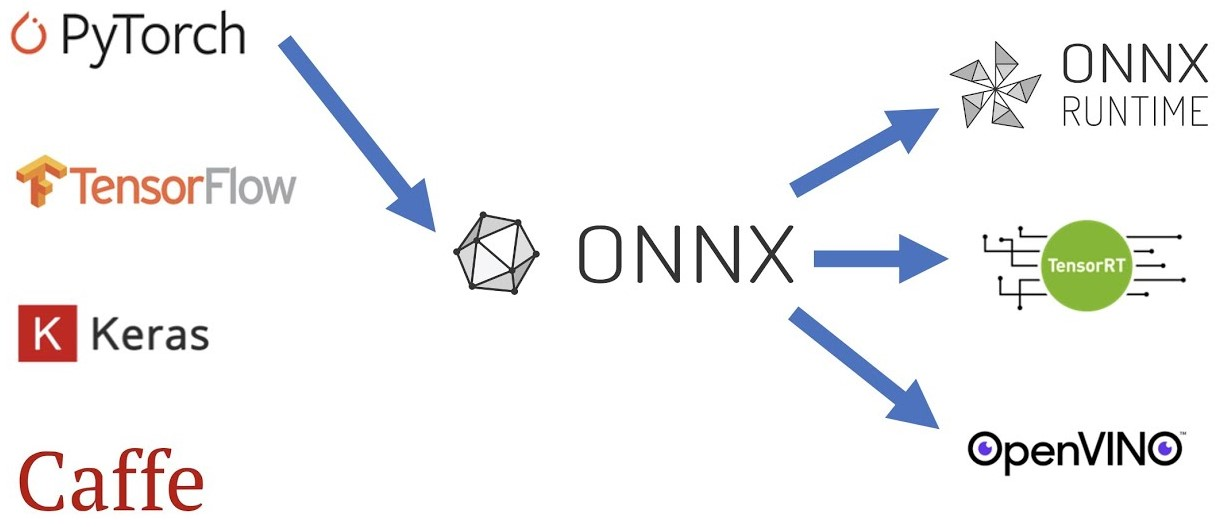
\includegraphics[scale=0.4]{gambar/pytorch-onnx-openvino.jpg}
  \caption{Flow of converting PyTorch Model to OpenVINO.}
  \label{fig:pytorch-to-openvino}
\end{figure}


\section{Choose Six Keypoints based on Humanoid Robot Keypoints}
\label{sec:choose-keypoints}

The difference in numbers between human keypoints and robot keypoints makes us have to choose certain human's keypoints in order to make a comparison between them.
Based on the results after testing, we chose Mediapipe for human and Keypoint RCNN for robot. Mediapipe provides 33 landmark keypoints for human and Keypoint RCNN only provides 6 keypoints.
Therefore, we need to choose 6 human keypoint as shown in Pseudocode \ref{lst:choose-human-keypoints}.
Note that, the name of the keypoints in the code corresponds to the name of the keypoints in the robot. First, we get all 33 keypoints. Then calculate the keypoint we want, such as the head keypoint which is located between the right and left eye.
To obtain the eye landmarks, we can index \verb|landmark| variable according to Figure \ref{fig:mediapipe-landmark}, where the left eye is index 2 and the right eye is index 5. This also applies to other landmarks.
The keypoint for the hands and feet is simply to select the wrists and ankles, where landmark[15] and landmark[16] are wrists, landmark[27] and landmark[28] are ankles.
Lastly, the trunk keypoint is located between the shoulder and hip keypoint. The x coordinate is located in the middle of the hip. The y-coordinate, on the other hand, is located on 1/4 distance between the hip and the shoulder from below.
First, we determine the midpoint between the shoulder and hip by individually calculating the coordinates of the right and left y axes, like Pseudocode \ref{lst:choose-human-keypoints} lines 19 and 21. In order to obtain 1/4 of the distance between the hip and the shoulder from below, we then compute the midpoint between the previous computation and the hip point as shown in lines 20, 22, and 24.
After all of the computation, we arrange all keypoints in a single array.

\lstinputlisting[
  language={},
  caption={Choose human keypoints.},
  label={lst:choose-human-keypoints}
]{program/choose-human-keypoints.txt}


\section{Keypoint Normalization}
\label{sec:keypoint-normalization}

When we think about the problem, we see that there are many uncertainties to be addressed. For example, human and humanoid robot can differ in height, body shape, and location within an image: one subject (human or robot) may have been nearby the camera,
while another may have been in the distance. In order to get an accurate outcome, each of these issues must be resolved.
After choosing the keypoints, the model output for both human and robot is the coordinates of 6 keypoints. This information can be used to create a new keypoint coordinates starting from (0,0) in the image. This solves the problem of the subject appearing in different parts of the picture.

\lstinputlisting[
  language={},
  caption={Get New Keypoints.},
  label={lst:new-keypoints}
  ]{program/bbox.txt}

In Pseudocode \ref{lst:new-keypoints}, the code is structured into two functions: \verb|get_min_point| and \verb|get_| \verb|new_coords|. The \verb|get_min_point| function takes an array of keypoints coordinates as input with shape (6,2)
and iterates through each item in the array. It keeps track of the minimum x and y values encountered during the iteration and returns an array containing the minimum x and y coordinates.
The \verb|get_new_coords| function takes the keypoint coordinates array and \verb|min_point| (minimum x and y coordinates) from the previous calculation as input. It iterates through each item and subtracts the corresponding minimum x and y values from each coordinate. The updated coords array is returned.

We further normalized the resulting keypoints coordinates by performing L2 normalization in order to transform it into a unit vector as shown in Figure \ref{fig:transforming-into-unit-vector}.
This means we are ignoring the size of the picture, but keeping in account the direction of the vector, created by the pose inside of that image.
To calculate the L2 normalization for an individual point is to take the square root of the sum of the squares of its coordinates. This calculation resulting the magnitude or length of the vector formed by the coordinates of the point.
Next step is dividing each coordinate by the length of the vector. This step ensures that the resulting normalized point lies on the unit circle. This normalization process scales the coordinates proportionally while preserving the direction of the vector. Moreover, it will optimize using NumPy library so it can compute multiple points simultaneously.

\begin{figure}[ht]
  \centering
  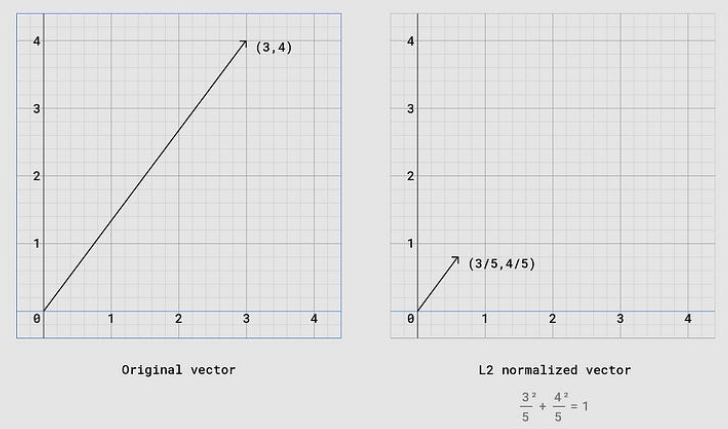
\includegraphics[scale=0.7]{gambar/transform-to-unit-vector.png}
  \caption{Transforming into Unit Vector.}
  \label{fig:transforming-into-unit-vector}
\end{figure}

\section{Comparing Human Keypoints and Robot Keypoints}
\label{sec:comparing-keypoints}

Now that we have standardized the pose vectors, it is time to choose a similarity measure. We chose cosine similarity for this particular instance, mainly because we are working with vectors and performing a few calculations detailed below to arrive at a Euclidean distance that can be interpreted as a cosine distance.
The cosine similarity ranges from -1 to 1, with 1 indicating identical poses or vectors are in the same direction, 0 indicating no similarity or vectors are nearly orthogonal, and -1 indicating completely opposite poses or opposite direction. The cosine distance, on the other hand, is a dissimilarity measure that ranges from 0 to 2.
Using Equation \ref{eq:euclideandistance} scales the values to the range of 0 to 2, making it easier to interpret the results. A larger value implies a greater dissimilarity between poses. In that equation, Fxy and Gxy are two pose vectors to be compared after L2 normalization. Moreover, Fxy and Gxy contain only x and y positions for each of the 6 keypoints, it does not include confidence scores.

\begin{equation}
  \label{eq:cosinesimilarity}
  cosineSimilarity(x,y) = \frac{x \cdot y}{|x||y|}
\end{equation}

\begin{equation}
  \label{eq:euclideandistance}
  D(F_{xy}, G_{xy}) = \sqrt{2 * (1 - cosineSimilarity(F_{xy}, G_{xy}))}
\end{equation}


\section{Pose Similarity Result}
\label{sec:pose-similarity-result}

The result of pose similarity is in percentages with a range of 0 to 100. A higher score indicates a more similar position between the human and robot, and vice versa.
In order to get it, we multiply the cosine distance result from Section \ref{sec:comparing-keypoints} by 100 and subtract the result from 100.
After getting each result of pose similarity, we take a mean and display it in the left top video. This video will be generated after detecting and comparing all poses.